\documentclass[12pt]{report}
\usepackage{indentfirst}
\usepackage{geometry}
\usepackage{flafter}
\usepackage{graphicx}
\usepackage{float}
\usepackage{titlesec}
\usepackage{tabularx}
\usepackage{relsize}

\graphicspath{ {./images/} }
\newgeometry{vmargin={15mm}, hmargin={28mm,28mm}}
\titleformat{\chapter}{\normalfont\huge}{\bf\thechapter.}{18pt}{\huge\bf}
\newcommand\ddfrac[2]{\frac{\displaystyle #1}{\displaystyle #2}}

\begin{document}

\begin{titlepage}
    \vspace*{4cm}
    \rule{\textwidth}{2px}

    \begin{center}
        \textbf{\huge{{Summer Practice Report }}}\par \vspace{0.2cm}
        \textbf{\Large{{TÜBİTAK İLTAREN}}}\par
    \end{center}
    
    \rule{\textwidth}{2px}
    
    \vspace{1cm}
    
    \begin{center}
        \large{Ahmet Eren Çolak - 2587921}
    \end{center}

    \vspace{1.3cm}
    
    \vfill
    \today
    
\end{titlepage}

\tableofcontents
\listoffigures
\listoftables

\chapter{Description of the Company}

    \section{Company Name}
    Scientific and Technological Research Council of Türkiye, Advanced Technologies Research Institute \\
    (TÜBİTAK İLTAREN)
    \section{Company Location}
    Ümitköy, 2432. Cad. 2489. Sok. Şehit Mu. Kur. Yzb. İlhan TAN Kışlası,
    Çankaya, Ankara 06800,
    Turkey.
    \section{Organizational Structure of the Company}

    \begin{figure}[h]
        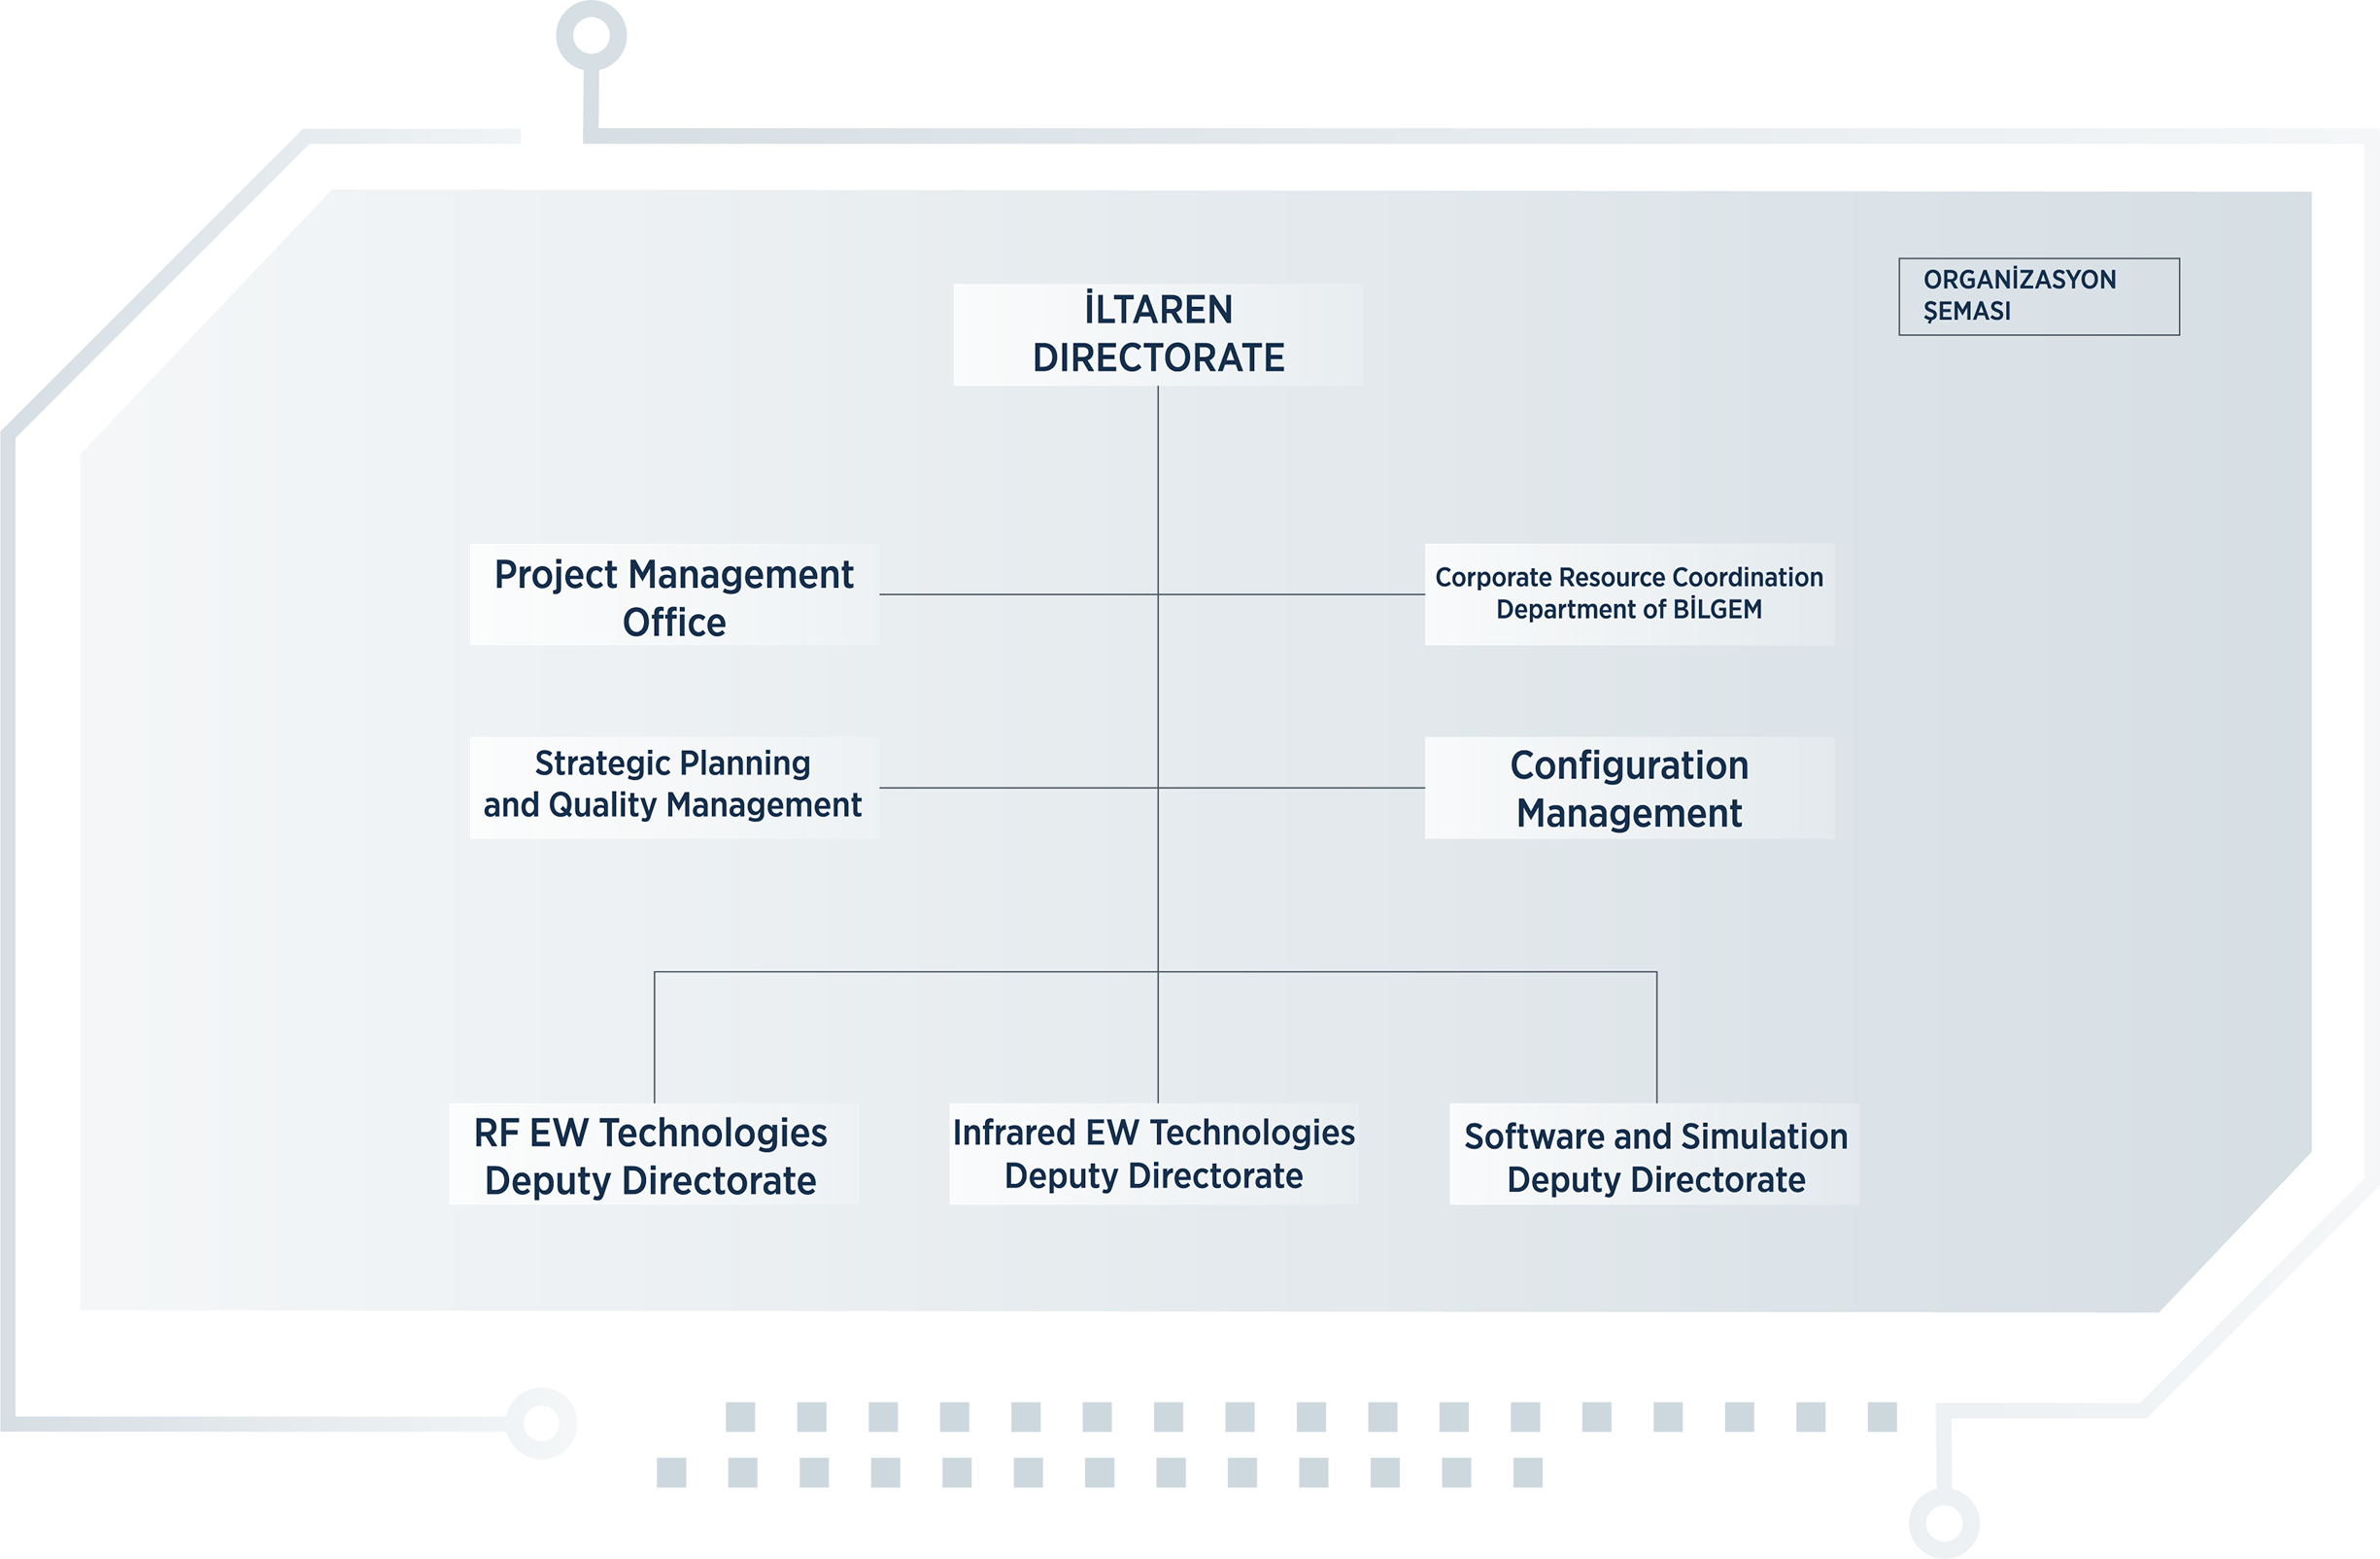
\includegraphics[scale=0.18]{iltaren-organization}
        \centering
        \caption{Organizational structure}
    \end{figure}

    \section{Number and Duties of Engineers Employed}
    Duties and number of employees can not be shared due to confidentiality policies of the company.
    
    \section{Main Area of Business}

    Advanced Technologies Research Institute (İLTAREN) performs the tasks of conducting research on all kinds of software, hardware and 
    equipment in the field of Electromagnetic Warfare, developing technologies and prototypes, creating methods and processes for developing 
    and evaluating EW techniques and tactics, creating infrastructures for testing, measurement, analysis and evaluation activities for 
    EW systems, and conducting scientific research in related fields of activity.

    \section{Brief History of the Company}
    The Advanced Technologies Research Institute (İLTAREN) is an organization based in Turkey that specializes in electronic warfare and advanced technology research. Here is a brief history of İLTAREN:
        \\ \newline
        \textbf{1999 - Establishment:} İLTAREN was established as a result of a protocol signed between the General Staff Communications Electronics and Information Systems Directorate and TÜBİTAK (The Scientific and Technological Research Council of Turkey). This protocol laid out the framework for cooperation in establishing the institute.
        \\ \newline
        \textbf{2000 - Inception:} İLTAREN officially began its activities under the TÜBİTAK Presidency in the year 2000. Its primary mission was to enhance the electronic warfare capabilities of the Turkish Armed Forces (TAF) through advanced research and technology development.
        \\ \newline    
        \textbf{2003 - Restructuring:} İLTAREN underwent restructuring, with the signing of a second protocol. It continued its operations as a unit within the National Research Institute of Electronics and Cryptology (UEKAE).
        \\ \newline
        \textbf{2007 - National Frequency Management System:} İLTAREN achieved a significant milestone with the development of the first version of the National Frequency Management System. This system is crucial for managing and allocating radio frequencies efficiently.
        \\ \newline
        \textbf{2010 - International Contributions:} İLTAREN developed the ARCADE product to meet NATO Spectrum Management needs and actively contributed to NATO Electronic Warfare exercises.
        \\ \newline
        \textbf{2011 - Infrared Trace Analysis Software:} İLTAREN developed Infrared Trace Analysis Software, which is likely a significant asset in the field of electronic warfare.
        \\ \newline
        \textbf{2012 - Engineering Support Contracts:} İLTAREN signed contracts with the Turkish Land Forces Command and NATO for engineering support in the field of electronic warfare and Spectrum Management needs, respectively.
        \\ \newline
        \textbf{2013 - İLTAREN Institute:} İLTAREN began to serve as an institute affiliated with BİLGEM (Informatics and Information Security Advanced Technologies Research Center).
        \\ \newline
        \textbf{2014 - Hardware Development:} İLTAREN continued its hardware development efforts, including the development of the Digital Tactical Simulator for Electronic Warfare self-defense.
        \\ \newline
        \textbf{2016 - Hardware In-Loop Laboratories:} İLTAREN expanded its capabilities with the development of Hardware In-Loop Laboratories for self-protection methods against both radio frequency (RF) and infrared systems.
        \\ \newline
        \textbf{2017 - Multi-Purpose Phased Array Radar Project:} İLTAREN contributed to radar technology development within the scope of the Multi-Purpose Phased Array Radar Project.
        \\ \newline
        \textbf{2018 - Instrumented Infrared Seeker Test System:} İLTAREN developed the Instrumented Infrared Seeker Test System, further advancing its expertise in infrared technology.
        \\ \newline
        \textbf{2019 - Engineering Support Agreement:} İLTAREN signed an agreement with the Turkish Air Forces Command to provide engineering support in the field of electronic warfare.
        \\ \newline
        \textbf{2020 - ESEMOD Software:} İLTAREN expanded the use of its ESEMOD software to work on MİLGEM class ships.
        \\ \newline
        \textbf{2021 - Jamming Code Development:} İLTAREN developed laboratory infrastructure for the development of jamming codes used in Directed Infrared Countermeasure Systems.
        \\ \newline
        \textbf{2022 - National Combat Aircraft Project:} İLTAREN played a role in the development of the integrated processor unit and avionic interface platform hardware for the National Combat Aircraft Project.
        \\ \newline
        \textbf{2023 - Radar Analysis Software:} İLTAREN delivered Radar Analysis Software for the National Joint Electronic Warfare Data Bank (MMEHBB) and celebrated the first functional flight of the Electronic Warfare Pod on the F16.
        \\ \newline
    Throughout its history, İLTAREN has consistently contributed to the advancement of electronic warfare technologies, Spectrum Management, and related fields, serving as a vital asset for the Turkish Armed Forces and international partners.

\chapter{Introduction}
    This report provides a summary of the work I have done and experiences I have gained during my 6-week summer 
    practice at the Advanced Technologies Research Institute (İLTAREN). 
    
    Throughout my internship at the Software and Simulation Deputy Directorate, I mainly worked on development of 
    algorithms for specific problems and implementation of data structures required for the implementation of algorithms.
    \newline

    Tasks I have accomplished can be inspected in three parts: 
    \begin{itemize}
        \item Implementation of statically allocated vector and linked list
        \item Approximation of the longest path in a graph
        \item De-interleaving radar pulses based on time of arrivals.
    \end{itemize}

    

\chapter{Project}
    \section{Longest Path in a Graph}
        \subsection{Analysis Phase}

            \textbf{Problem Definition:} There exists a CSV file which contains distances from 81 cities of Turkey to all other 81 cities in Turkey. 
            Using this distance matrix read from that CSV file, you are expected to compute the maximum amount of city that can be traveled 
            (without visiting a city twice) only using the roads which its distances are in the interval of $[x-y, x+y]$. The values $x$ (distance) and $y$ (tolerance) 
            are given by the user.
            \newline

            Example CSV file format:

            \begin{verbatim}
                ADANA;ADIYAMAN;AFYONKARAHISAR;AGRI;AMASYA;ANKARA;  ...
                01;ADANA;0;338;579;978;604;492;548;1005;881;903;78 ...
                02;ADIYAMAN;338;0;917;646;628;738;886;717;1219;124 ...
                03;AFYONKARAHISAR;579;917;0;1320;596;255;287;1225; ...
                04;AGRI;978;646;1320;0;740;1056;1426;365;1635;1576 ...
                05;AMASYA;604;628;596;740;0;331;824;679;936;842;62 ...
                06;ANKARA;492;738;255;1056;331;0;543;960;596;536;3 ...
                07;ANTALYA;548;886;287;1426;824;543;0;1433;346;506 ...
                08;ARTVIN;1005;717;1225;365;679;960;1433;0;1565;14 ...
                09;AYDIN;881;1219;340;1635;936;596;346;1565;0;291; ...
                10;BALIKESIR;903;1241;324;1576;842;536;506;1452;29 ...
                11;BILECIK;786;1039;207;1361;626;314;473;1236;525; ...
                12;BINGOL;633;348;1099;352;642;889;1191;373;1401;1 ...
                13;BITLIS;746;414;1290;232;833;1080;1294;547;1592; ...
                14;BOLU;689;927;417;1146;411;190;683;1021;735;431; ...
                ...
            \end{verbatim}

            When the distances which does not fit in the interval of $[x-y, x+y]$ are replaced with the zero $(0)$ and the rest is set to one $(1)$, distance matrix becomes into a 
            adjacency matrix of an unweighted graph. Then the goal becomes into computing the longest path in that graph. How dense or how sparse the graph is controlled by the 
            tolerance variable ($y$), and combinations of edges in the graph is adjusted by the distance variable ($x$).
            
            Finding an exact solution to this problem requires comparing all different 
            permutations of cities and checking whether they form a path. This process requires comparison of $n!$ different orderings. Therefore it is not possible
            to find an exact solution to this problem in a polynomial time. When the case with our problem is considered where $n=81$ and $n! \approx 5.8\cdot 10^{120}$,
            computation of an exact solution may take many months even for a modern computer.

            Therefore, computing an approximate solution in polynomial time rather than an exact solution is much more feasible. To compute an approximation of the
            longest path, I decided to follow a heuristic approach where the locally optimum neighbouring city is chosen to continue with at each iteration. This therefore
            raises the question of what kind of heuristics should be used for choosing an ideal local optimum at each step ?

        \subsection{Design Phase}
            
            Assume that we are looking for a long path in the unweighted and undirected graph $G=(V,E)$, starting from the vertex $s \in V$. Let $N$ be the set of all vertices
            which have an edge with vertex $s$, in other words $N$ is the set of neighbours of $s$. 
            \newline

            Then the process of approximating a long path in graph $G$ follows as:

            \begin{enumerate}
                \item Compute a score value for each vertex in $N$.
                \item Choose the vertex with the maximum score.
                \item Update $N$ as the set of neighbours of the chosen vertex.
                \item Go to $1$ until there is no vertex left to visit.
            \end{enumerate}

            Computing the score for a vertex is the most critical task which entirely determines the performance of the algortihm and the length of the approximated path. 
            Heuristic functions should be chosen such that even when the graph is sparse (which means tolerance variable $y$, is low) algorithm should not perform poorly. 
            \newline

            First thing I thought was the direct neighbour count of the vertices. Idea of choosing the vertex with the most neighbours leads to longer paths, seems reasonable at 
            first sight however it is not. Because choosing the vertices with most neighbours repetitevely, leaves out the vertices with few neighbours. That makes it hard for visiting
            vertices with few connections in the future. Although this heuristic does not seem useful right now, it can be helpful for the solution of the problem as I am going to 
            explain later.

            Since count of direct neighbours is known to be a poor choice of heuristic for finding long paths, it can be thought that maximum count of second order neighbours may 
            perform better. Maximum count of second order neighbours, is the maximum of count of direct neighbours which a vertex's direct neighbour has. On average, it actually 
            performs better than the count of direct neighbours.

            Observation of the increase in the performance with looking deeper in the graph for the count of neighbours, leads to trial of maximum count of the third and forth order neighbour 
            counts. Maximum count of third order neighbours, is the maximum of count of second order neighbours which a vertex's direct neighbour has. Same idea applies for the
            definition of the forth order neighbours. Although choosing the heuristic as the maximum count of third order neighbours performs better than the heuristic of maximum 
            count of the second order neighbours, when heuristic is chosen to be the maximum count of the forth order neighbours it performs poorer than the third order one. 
            Decrease in the performance continues as the order of neighbours are increased which is used in the heuristic.
        
            Since heuristics related to neigbour counts can not be improved any more, I looked for different kinds of metrics of graphs. Centrality metrics which gives information
            about the positions of vertices in the graph, may be useful for finding long paths. Motivation of using indicators of centrality originates from the idea that long paths
            tend to contain more vertices which are positioned at the central regions of the graph.   

            Closeness centrality is one of the methods to measure centrality of a vertex in a graph. Closeness centrality or closeness of a vertex is the average length of the 
            shortest path between the vertex and all other vertices in the graph. Thus the more central a vertex is, the closer it is to all other nodes.
            Closeness centrality of a vertex $v$ is computed as below where $d(u,v)$ is the shortest distance between vertices $u$ and $v$:
            
            \bigskip
            \begin{equation}
                C(v) = \ddfrac{1}{\sum_{u \in V} d(u,v)}
            \end{equation}
            \bigskip

            Another measure of centrality is the betweenness centrality. Betweenness centrality is the measurement of how many times a vertex acts as a bridge between shortest 
            path of any two vertices in the graph. Vertices which are at the central regions tend to be contained in many paths in the graph, because of this number of times a
            vertex being in any paths in graph is a measurement of centrality. Betwenness centrality of vertex $v$ is computed as below, where $\sigma_{st}$ indicates the total
            number of shortest paths from node $s$ to $t$ and $\sigma_{st}(v)$ is the number of those paths which contains vertex $v$.

            \bigskip
            \begin{equation}
                C_B(v) = \sum_{s \neq t \neq v \in V} \ddfrac{\sigma_{st}(v)}{\sigma_{st}}
            \end{equation}
            \bigskip

            \begin{figure}[h]
                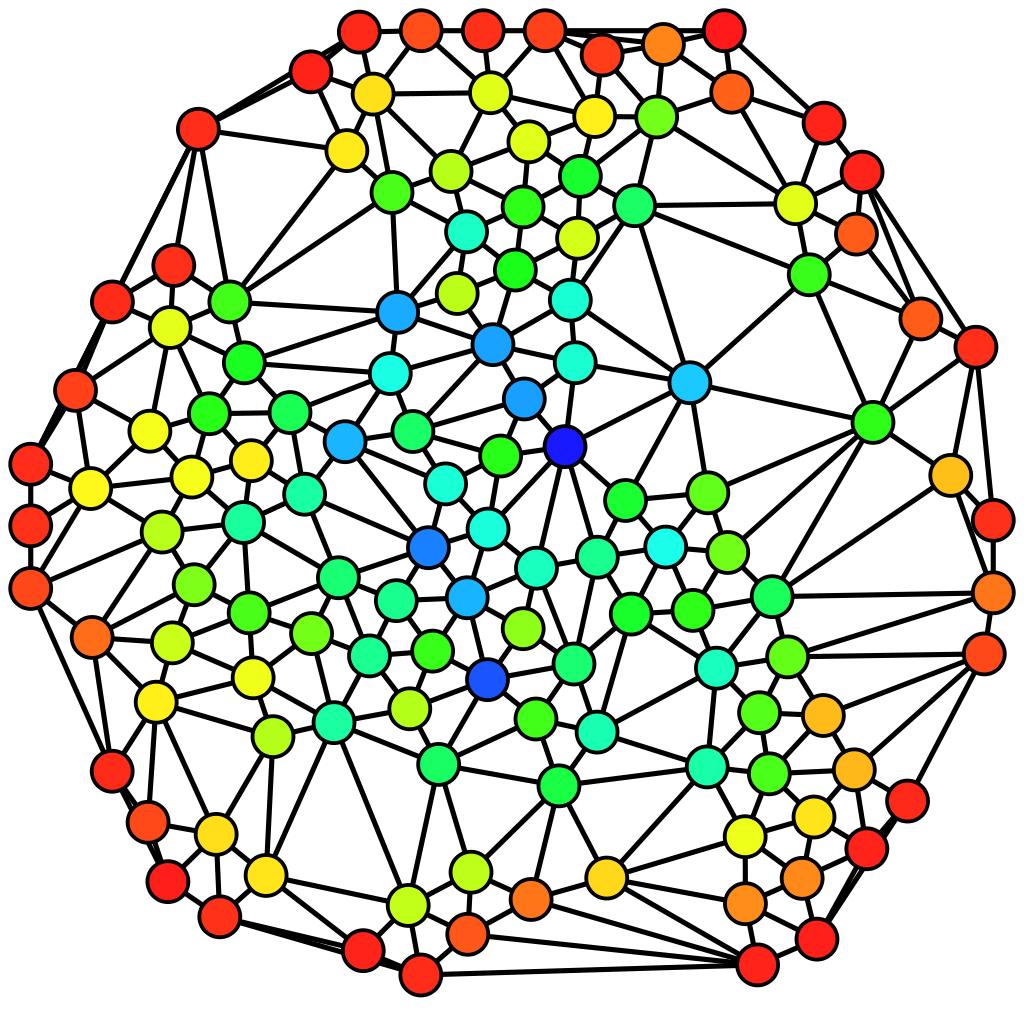
\includegraphics[scale=0.25]{betweennes-centrality}
                \centering
                \caption{Betweenness centrality of vertices in a graph}
            \end{figure}
            \bigskip

            Apart from the centrality metrics, another heuristic approach for searching long paths could be considering the total length up to vertices which are available to be chosen.
            Rationale for this method is that as algorithm iterates further, it may get harder to visit closer vertices to the starting vertex of the travel. 
            Therefore choosing the vertex which is closest to starting vertex may lead to longer paths.
            
            An alternative of distance to starting vertex heuristic is considering the distance to previously visited vertex. Aim is to choosing the vertex which is closest to previously
            visited vertex, thus leading a long path in graph. Downside of this heuristic compared to distance to previous heuristic is that there are only two score values for a vertex.
            The score is either $1$ or $2$. Because, score of a vertex is $1$ if and only if a vertex has a direct edge with the previously visited vertex. Otherwise it's score is always $2$, 
            since shortest path from that vertex to previously visited vertes has to contain only the current vertex of the iteration. Therefore this approach may fail to distinguish multiple
            neighbours of a vertex, when compared with the distance to previous heuristic.
            \newline



        \subsection{Implementation Phase}

        \subsection{Testing Phase}

    \section{Radar Pulse De-interleaving}
        \subsection{Analysis Phase}

        \subsection{Design Phase}

        \subsection{Implementation Phase}

        \subsection{Testing Phase}

\chapter{Organization}

    \section{Organization and Structure}

    \section{Methodologies and Strategies Used in the Company}

\chapter{Conclusion}

\chapter{Appendix}

\end{document}